\chapter{Introduction}
\label{chap:intro}

\section{The Expansion History of the Universe}
Understanding how space has expanded over the history of the universe is key to understanding what the universe is made of, how it started, and how it may end. We start by defining the scale factor, $a$, which describes the ratio of the physical distances between objects in the past to the physical distances between the same objects today. Our quest to measure the expansion history of the universe, then, is equivalent to determining $a(t)$ -- how the scale factor evolves with cosmic time.

The cosmological principle descends from the Copernican principle: that there is nothing special about our particular viewpoint of the universe. More precisely, it states that the expansion of the universe is homogenous (the same at any point in space) and isotropic (the same in all directions). Encoding this mathematically, we can obtain the following metric, known as the Friedmann-Lema\^{i}tre-Robertson-Walker (FLRW) metric:
\begin{equation}
    ds^2 = a(t)^2\,ds_3^2 - c^2\,dt^2
    \label{eqn:flrw_metric}
\end{equation}
where $ds_3$ is the three-dimensional spatial metric and $c$ is the speed of light.

Using this metric in the Einstein field equations, we then derive the Friedmann equations, a general description of how $a$ evolves with time:
\begin{equation}
    \left(\frac{\dot{a}}{a}\right)^2 = \frac{8\pi G\rho}{3} - \frac{kc^2}{a^2}
    \label{eqn:friedmann}
\end{equation}
\begin{equation}
    \frac{\ddot{a}}{a} = -\frac{4\pi G}{3}\left(\rho + \frac{3p}{c^2}\right)
    \label{eqn:friedmann_acceleration}
\end{equation}
Dots here represent a time derivative, and $G$ is Newton's gravitational constant. The energy density, represented by $\rho$, and the energy pressure, $p$ are functions of time, like the scale factor $a$. The spatial curvature, $k$, is constant, but can take on a number of values.

To simplify our notation, we define the Hubble rate:
$$H=\frac{\dot{a}}{a}.$$
With this, the left hand side of Equation \ref{eqn:friedmann} can be replaced with $H^2$ and the left hand side of Equation \ref{eqn:friedmann_acceleration} can be replaced with $\dot{H} + H^2$.  The value of the Hubble rate today is known as the Hubble constant, $H_0$.

Assuming $k=0$ (an assumption that is experimentally justified from observations of the cosmic microwave background, see \citet{planck_collaboration_planck_2016}, for example), we can use Equation \ref{eqn:friedmann} to rewrite Equation \ref{eqn:friedmann_acceleration} as
\begin{equation}
    \dot{\rho} = -3H\left(\rho + \frac{p}{c^2}\right)
    \label{eqn:density_evol}
\end{equation}
For linear combinations of perfect fluids, each with equation of state
$$p_f = w\rho_f c^2$$
(where $w$ is known as the equation of state parameter), this equation has exact solutions of the form
$$\rho_f \propto a^{-3(1+w)}.$$
For ordinary matter, $w=0$. For radiation, $w=1/3$ and for a cosmological constant dark energy, $w=-1$. Thus, Equation \ref{eqn:density_evol} has solutions of the form:
$$\rho = \rho_m a^{-3} + \rho_r a^{-4} + \rho_\Lambda$$
Additionally, we define the critical density
$$\rho_{c} = \frac{3H_0^2}{8\pi G},$$
which describes the average energy density of a universe that would halt expansion after infinite time. Dividing the densities by this critical density gives us a unitless density parameter $\Omega$. Putting everything, together, we can obtain the relationship between the Hubble parameter and scale factor, parametrized by the time-evolving densities of the constituent components of the universe:
\begin{equation}
    H(a) = H_0\sqrt{\Omega_m a^{-3} + \Omega_r a^{-4} + \Omega_\Lambda}
    \label{eqn:hubble_vs_a}
\end{equation}
% Proof:
% $$H^2 = \frac{8\pi G}{3}\rho$$
% $$2H\dot{H}=\frac{8\pi G}{3}\dot{\rho}$$
% $$\dot{H}=\frac{4\pi G}{3H}\dot{rho}$$
% $$\dot{H} + H^2 = -\frac{4\pi G}{3}\left(\rho + \frac{3p}{c^2}\right)$$
% $$\frac{4\pi G}{3}\left(\frac{\dot{\rho}}{H} + 2\rho\right) = -\frac{4\pi G}{3}\left(\rho + \frac{3p}{c^2}\right)$$
% $$\dot{\rho} = -3H\left(\rho + \frac{3p}{c^2}\right)$$

Oftentimes, it is convenient to use the redshift, $z$, in lieu of the scale factor, since the redshift is directly observable. We define the redshift as the Doppler-like shift observed in distant objects:
\begin{equation}
    z = \frac{\lambda_o}{\lambda_e} - 1
    \label{eqn:z_def}
\end{equation}
where $\lambda_o$ is the observed wavelength and $\lambda_e$ is the emitted wavelength of some observable spectral line. The redshift we observe has a number of source. For our purposes, the main contributors are the cosmological redshift, where the expansion of space stretches of the wavelength of emitted light causing it to appear redder, and the peculiar velocity redshift, where the motion of objects relative to us creates a Doppler shift in the observed wavelengths. Generally, when we refer to the redshift of an object, we are referring to its cosmological redshift, which is related to the scale factor by $z = 1/a - 1$. Using this definition in Equation \ref{eqn:hubble_vs_a}, we get
\begin{equation}
    H(z) = H_0\sqrt{\Omega_m (1+z)^{3} + \Omega_r (1+z)^{4} + \Omega_\Lambda}
\end{equation}

We're now in a position to begin to define some useful measures of cosmological distance, using the equations that govern the evolution of distances described above. One important distance measure for the work described here is the comoving distance, $\chi$, between an emitting object at scale factor $a$ and us ($a=1$). This distance remains constant with the universe's expansion and can be calculated by multiplying the speed of light with the aggregate of infinitesimal distances over time:
\begin{equation}
    \chi = c\displaystyle\int_{t(a)}^{t_0} \frac{dt^\prime}{a(t^\prime)}
    = -c\displaystyle\int_1^a \frac{da'}{a'^2 H(a)}
    = \frac{c}{H_0}\displaystyle\int_0^z \frac{dz'}{\sqrt{\Omega_m(1+z')^3 + \Omega_r(1+z')^4 + \Omega_\Lambda}}
\end{equation}

The angular diameter distance describes the ratio of an object's physical size to its angular size on the sky, and is related to the comoving distance by
$$d_A(z) = \frac{\chi(z)}{1+z}$$

Finally, we have the most important distance measure for our work: the luminosity distance. This distance defined by
\begin{equation}
    d_L(z) = \sqrt{\frac{L}{4\pi F}}
    \label{eqn:luminosity_dist}
\end{equation}
where $L$ is the luminosity of an object and $F$ is the flux (or observed brightness) of the object. Interestingly, it can be shown that this quantity is equivalent to \footnote{The full proof of this equivalence (known as the Etherington reciprocity theorem) is quite complicated. However, we can obtain this relation by noting that the surface brightness of an object is reduced by a factor of $(1+z)^{-4}$ as it recedes, while the angular area decreases as $d_A^{-2}$ \cite{hogg_distance_1999}.}
\begin{equation}
    d_L(z) = (1+z)^2 d_A(z) = (1+z)\chi(z).
    \label{eqn:luminosity_dist_z}
\end{equation}


In astrophysical contexts, it is common to work in logarithmic-scale magnitudes. This leads to the definition of the distance modulus, $\mu$ defined as the difference between the apparent magnitude of an object, $m$, and its absolute magnitude, $M$ which is itself defined as the apparent magnitude of an object if it were seen from a distance of 10 parsecs. The distance modulus is therefore related to the luminosity distance by
\begin{equation}
    \mu = m - M
    = -2.5 \log_{10}\left[\frac{F(d_L)}{F(d_L = 10\textrm{ pc})}\right] = 5 \log_{10}\left(\frac{d_L}{10\textrm{ pc}}\right) - 5
    \label{eqn:distmod}
\end{equation}

\section{Using Standard Candles to Constrain Cosmological Parameters}
A classic method for obtaining estimates of the luminosity distance is to observe standard candles. A standard candle is any class of astronomical objects that has a known intrinsic luminosity. By observing the apparent brightness of these objects, we directly obtain the luminosity distance as defined in Equation \ref{eqn:luminosity_dist} (or equivalently the distance modulus as defined in Equation \ref{eqn:distmod}). We can also use spectral observations of these objects or their host galaxies to compare the observed frequencies of various emission and absorption lines in the spectrum to the known frequencies of these lines in order to calculate each object's redshift, as in Equation \ref{eqn:z_def}. Combining these measurements gives us the Hubble-Lema\^{i}tre diagram, a plot of luminosity distance (or equivalently the distance modulus) as a function of redshift. Different cosmological models predict different relationships between distance and redshift, so our standard candle observations can be used to differentiate between and constrain the parameters of different theoretical models. In Figure \ref{fig:hubble_diagram_examples}, we show a few examples of distance-redshift relations for different cosmological models.

\begin{figure}[htpb]
    \centering
    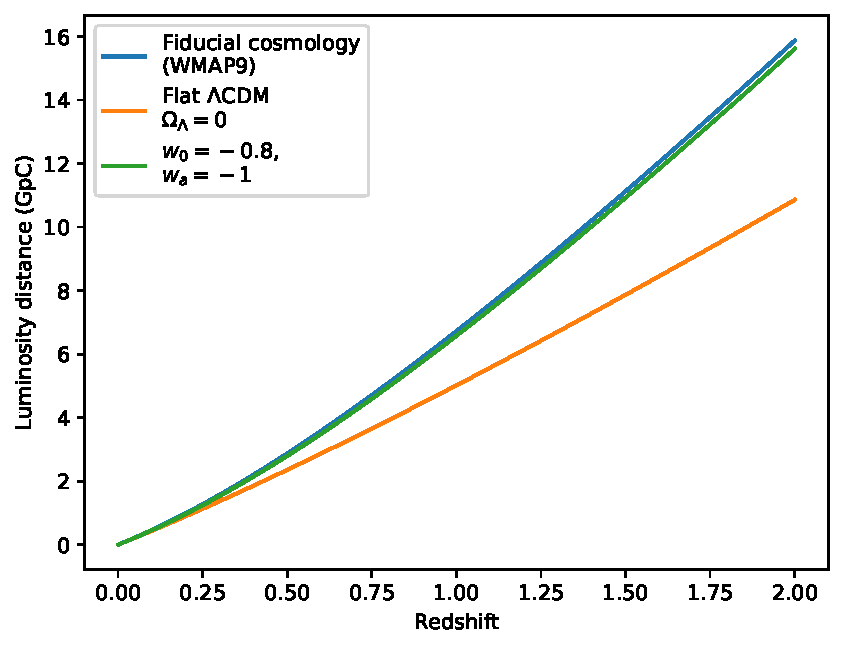
\includegraphics{figures/intro/hubble_diagram_examples.pdf}
    \caption{Hubble-Lema\^{i}tre diagrams for different cosmological models. In blue, we have a fiducial, flat $\Lambda$CDM cosmology with density parameters matching those determined by \citet{komatsu_five-year_2009}. In orange, we show another flat $\Lambda$CDM cosmology, but dominated entirely by matter (i.e. $\Omega_\Lambda=0$). In green, we show an example of the distance-redshift relation for an alternate parametrization of dark energy with a varying equation of state parameter.}
    \label{fig:hubble_diagram_examples}
\end{figure}

The standard cosmological model is the flat, $\Lambda$CDM model, which posits that the spatial curvature of the universe is flat ($\Omega_k=0)$, and that the energy density is composed primarily of dark energy that behaves as a cosmological constant, followed by cold dark matter, and finally ordinary baryonic matter. This model is supported by the findings of a number of different probes \citep{planck_collaboration_planck_2016, wittman_detection_2000, eisenstein_detection_2005}. Its Hubble-Lema\^{i}tre diagram is shown in blue in Figure \ref{fig:hubble_diagram_examples}, where we have take the density parameter values from \citet{komatsu_five-year_2009}: $\Omega_\Lambda = 0.7135$ and $\Omega_m = 0.2865$. We can see that the distance-redshift relation for this cosmology differs significantly from a similarly parametrized cosmology but with $\Omega_\Lambda=0$ and $\Omega_m=1$ (seen in orange in Figure \ref{fig:hubble_diagram_examples}).

$\Lambda$CDM is not the only cosmological model. One popular alternate model envisions dark energy as a dynamical scalar field, rather than a cosmological constant. In this case, the equation of state parameter $w$ of dark energy is allowed to vary with redshift (or equivalently, scale factor). This variation can be parametrized by
\begin{equation}
    w(a) = w_0 + w_a(1 - a) = w_0 + w_a z/(1+z)
\end{equation}
(see \citet{chevallier_accelerating_2001} or \citet{linder_exploring_2003}). A cosmological constant can be encapsulated by this parametrization by setting $w_0=-1$ and $w_a=0$, so deviations from these values would serve as useful clues as to the precise nature of dark energy. An example distance-redshift relation with $w_0=-0.8$ and $w_a=-1$ is shown in green in Figure \ref{fig:hubble_diagram_examples}. We can see that the difference in the current fiducial cosmology distance-luminosity relationship and that of this alternate cosmology is quite small, but increasing with redshift. In order to constrain the parameters of these alternate models, we need to have extremely precise measurements of the luminosity distance, and also be able to extend these measurements further back in time (i.e. to higher redshift).

\section{Type Ia Supernovae as Standardizable Candles}
\label{sec:standardizable_candles}
Type Ia supernovae (SNe Ia), exploding carbon-oxygen white dwarfs in binary systems, are excellent standard candle candidates. They are observed to have very similar intrinsic brightnesses. Moreover, they are extremely bright — about 5 billion times brighter than the Sun — so they can be seen out to large distances, and therefore probe earlier epochs of cosmic history. SNe Ia were instrumental in discovering that the expansion rate of the universe is accelerating, and they remain one of the best tools we have for constraining the properties of the dark energy that drives this accelerating expansion \citep{perlmutter_measurements_1999, riess_observational_1998}.

While Type Ia supernovae do have similar intrinsic brightnesses, they are not perfect standard candles. The scatter in their peak absolute magnitudes is $\sim 40$\%. They are, however, standardizable candles; that is, their peak brightnesses are strongly correlated with other observable properties of the explosion.

One of these observables is the light curve width (sometimes referred to as the decline rate), a measure of how quickly the event brightens and fades. SNe Ia with broader light curves tend to be intrinsically brighter. The relationship was first shown empirically in the 1970s \citep{rust_use_1974, pskovskii_light_1977} and later refined with additional observations and extending out to higher redshifts \citep{phillips_absolute_1993, hamuy_morphology_1996, perlmutter_measurements_1997}. The color of the supernova is also known to correlate with the brightnesses of SNe Ia -- bluer objects tend to be brighter. The width-luminosity relationship is theoretically explained as being due to differences in the opacity due to temperature differences \citep{kasen_origin_2007}. The color-luminosity relationship is not yet well-explained theoretically, but has been reproduced in a number of theoretical models \citep[e.g.][]{kasen_diversity_2009}. \citet{tripp_two-parameter_1998} introduced the combined correction for both width and color, enabling Type Ia supernova magnitudes to be standardized to within approximately 0.15 magnitudes, and similar relationships have been used in models like the multicolor light curve shapes model \citep[MLCS,][]{riess_precise_1996}.

Currently, the conventional method for standardization involves fitting observed broadband light curves with the SALT2 model of \citet{guy_salt2_2007} in order to obtain measurements of the light curve width and the color. SALT2 does not directly measure the light curve width or color like previous methods, which use parameters like $\Delta m_{15}$, the decrease in Bessell B-band magnitudes from maximum light to 15 days after maximum. Instead, the model parametrizes the full evolution of the spectral fluxes of Type Ia supernovae as follows:
\begin{equation}
    f(\lambda, p) = x_0\left(M_0(\lambda, p) + x_1 M_1(\lambda, p)\right) \times \exp [c\times\textrm{CL}(\lambda)]
    \label{eqn:salt_flux}
\end{equation}
where $\lambda$ represents wavelength and $p$ is the number of rest-frame days after maximum brightness (also known as the phase). $M_0$ and $M_1$ are fixed spectral sequences that describe the mean spectral evolution of SNe Ia and their major sources of spectral variation, respectively. $\textrm{CL}(\lambda)$ is a fixed description of the color variation that remains fixed across phases, and includes contributions from both intrinsic color differences and color differences due to host galaxy dust extinction. This model can be thought of as akin to a principal component decomposition of SN Ia spectral evolution, with $x_0$, $x_1$, and $c$ indicating where each supernova is located in the model basis and representing each supernova's overall brightness, light curve width, and redness, respectively. Using such parametrization avoids systematic errors from K-corrections that stem from large variations in spectral features.

After using the model to fit each supernova in a given data set, we typically standardize their observed brightnesses using a modified version of the Tripp relation:
\begin{equation}
    \mu = m_B^* - M + \alpha \times x_1 - \beta\times c
    \label{eqn:standardization}
\end{equation}
where $m_B^*$ is the apparent B-band magnitude calculated from the best-fit model parameters $x_0$, $x_1$, and $c$ for each supernova and $\mu$ is the distance modulus to each supernova. $M$, $\alpha$, and $\beta$ are global parameters that describe the overall standardized absolute magnitude in the  Bessell B-band, the light curve shape-luminosity relation, and the color-luminosity relation, respectively. Typically, we start by assuming some fiducial cosmology that defines a distance $\mu_\text{cosmo}$, and we fit the global standardization parameters $M$, $\alpha$, and $\beta$ by minimizing the $\chi^2$ defined by
\begin{equation}
    \chi^2 = (\mu - \mu_\text{cosmo})^T C^{-1} (\mu - \mu_\text{cosmo}),
    \label{eqn:chi2_cosmo_full_cov}
\end{equation}
where $C$ defines the covariance matrix between SN Ia observations. Then by fixing these values of $M$, $\alpha$, and $\beta$, we can perform a similar $\chi^2$ minimization that finds the best-fit cosmological parameters. The process repeats until convergence.

Alternatively, the UNITY framework \citep{rubin_unity_2015} performs this standardization and cosmology fit from light curve parameters with a fully Bayesian approach. In this case, the nuisance parameters and cosmological parameters, as well as their full posterior distributions, are obtained using Hamiltonian Monte Carlo techniques.

Regardless of the method of fitting, the residuals on the Hubble diagram (i.e. the differences between the distance moduli obtained from the best standardization of the light curve parameters and the distance moduli predicted by the best-fit cosmological parameters) still have a root-mean-square (RMS) dispersion of approximately 0.15 magnitudes. Some of this dispersion can be explained by the measurement, calibration, and model uncertainties of the photometry and light curve model fitting process. However, some amount of the dispersion (typically about 0.10 magnitudes) remains unexplained.

\section{SN Ia Standardization Beyond SALT2}
The remaining unexplained dispersion in standardized supernova magnitudes from using SALT2 and the Tripp relation indicates that there may be more progress to be made in SN Ia standardization. One method to make such an improvement is to look for additional parameters that correlate with the remaining variation and using these to correct the residuals further. \citet{kelly_hubble_2010} and \citet{sullivan_dependence_2010} found evidence of such a correlation between the host galaxy mass of supernovae and their Hubble residuals. Because of this, it is now standard to see supernova cosmology analyses include a correction term in their distance moduli calculations to account for this correlation. It has also inspired the search for other corrections to supernova magnitudes stemming from the supernova environment, like examinations of the global (entire galaxy) or local specific star formation rate \citep{rigault_evidence_2013, rigault_confirmation_2015}.

Some of these additional parameters are measured from the supernovae themselves, rather than their environments. A number of studies have searched for correlations between supernova spectral features and their absolute luminosities. \citet{nugent_evidence_1995} first outlined the existence of a spectroscopic sequence that relates the ratios of the depths of the \ion{Si}{ii} $\lambda$6355 and \ion{Si}{ii} $\lambda$5972 lines and the ratios of the \ion{Ca}{ii} H\&K lines to the absolute magnitude. \citet{bailey_using_2009} used the ratio of the absolute fluxes at two specific wavelengths to improve the standardization beyond what was possible with the Tripp standardization. Other studies have attempted to subclassify Type Ia supernovae using spectral indicators like the width of the \ion{Si}{ii} $\lambda$6355 and \ion{Si}{ii} $\lambda$5972 lines \citep{branch_comparative_2006}, or the ejecta velocity as measured by the blue shift of the minima of these lines \citep{wang_improved_2009, foley_measuring_2011, foley_relation_2012}. By using different corrections for these subclasses, these studies have shown some improvements to the standardization precision.

An alternate approach is to create more flexible light curve or spectral models. This is the tack taken by the SNEMO models \citep{saunders_snemo_2018}. SNEMO extends the logic of SALT2 by modeling the full spectral time series evolution of SNe Ia fluxes with additional components beyond the light curve shape captured by SALT2's $x_1$ parameter. The SNEMO flux model is
\begin{equation}
    f(\lambda, p) = c_0\left[e_0(\lambda, p) + \displaystyle\sum_{i=1}^k c_i\times e_i(\lambda, p)\right] \times \exp\left[A_s\times \textrm{FM07}(\lambda)\right]
\end{equation}
where $\textrm{FM07}$ is the \citet{fitzpatrick_analysis_2007} dust extinction law. The functional form of this equation is quite similar to that of Equation \ref{eqn:salt_flux}, however the number of linear components, $k$, is not fixed to one. SNEMO encompasses three separate models, each varying in the number of linear components that are used, and each intended for different uses. SNEMO2 ($k=1$) is useful as a comparison to the typical light curve shape and color models like SALT2, as the training methodology is slightly different from that of SALT2. SNEMO15 ($k=14$) was introduced as a model that captures as much of the spectral variation that exists in Type Ia supernovae without overfitting. The SNEMO7 model is intended as an intermediate model that can best standardize SN Ia magnitudes, using an extension of the Tripp relation:
\begin{equation}
    \mu = m_B - \left(M + \beta A_s + \displaystyle\sum_{i=1}^k \alpha_k \; c_k\right)
\end{equation}
The resulting dispersion with this parametrization is approximately 0.113 mag, of which 0.097 magnitudes are not explained by the measurement error. Thus, by extending the model used to describe supernova spectral variation, SNEMO is able to improve the standardization precision.

The SUGAR model presented in \citet{leget_sugar_2020}, effectively combines both approaches -- using spectral feature measurements as an alternate parametrization of a full spectral time-series model. Rather than performing a principal component decomposition of the full, interpolated, spectral time-series data (like SNEMO), SUGAR first measures a series of spectral indicators in the near-maximum spectra. Then, a PCA decomposition of these indicators is used to obtain a 4-dimensional projection vector corresponding to each supernova in the data set. Finally, the full spectro-temporal model is created by fitting for basis functions like the $e_i(\lambda, p)$ of SNEMO that, when linearly combined with the spectral indicator projections, accurately predict the spectral evolution of the supernovae. The SUGAR model does not yet have a corresponding standardization model, so we do not yet have an estimate of how well we can correct the brightnesses of supernova for the effects captured by the SUGAR model. However, the model is able to capture much more of the spectral variation in SNe Ia than SALT2, without a large increase in the number of parameters in the model.

So far, all of the methods discussed have been parametric and model both the spectral evolution (besides color) and the relation between SN parameters and SN absolute luminosities linearly. The work of \citet{fakhouri_improving_2015} takes a non-parametric approach, directly comparing the spectra of supernovae to identify pairs of ``twins," i.e. supernovae with nearly identical spectral time-series data, up to a difference in host-galaxy dust extinction and apparent magnitude. They found that the best pairs of twins differed in absolute magnitude on average by only $0.083 \pm 0.012$ mag (and by only $0.072 \pm 0.010$ mag after accounting for peculiar velocities). This implies that a direct comparison of the spectra, without any intermediate parametrization and modeling of necessary corrections, could produce better standardization.

\citet{boone_twins_2020a} sought to understand the mathematical structure of the ``twinness space" amongst near-maximum-brightness spectra. First, they estimated the aspects of the spectral variation that were due to differences in dust extinction and the overall brightness difference. Then, using the at-max spectra corrected for the differences in brightness and extinction, they applied the Isomap algorithm \citep{tenenbaum_global_2000} to find a low-dimensional representation of the remaining spectral variation that approximately preserves the twins distances from \citet{fakhouri_improving_2015}. The low-dimensional embedding faithfully reconstructs many of the previously discussed spectral indicators of supernova diversity. Furthermore, \citet{boone_twins_2020b} presents an additional model that predicts the variation in a supernova's brightness based on its location in the ``twins embedding." Using this technique, they were able to standardize the supernovae in the sample to within $0.084 \pm 0.007$ mag, a level comparable to the best twins comparison of \citet{fakhouri_improving_2015}, but with a parametric approach.

\section{Open Questions in Supernova Cosmology}
\subsection{Optimal Parametrization of SNe Ia}
We could see in the previous section that there has been much work put into the development of empirical models of Type Ia supernova spectral variation and evolution, including linearly parametrized models of the full spectral evolution (SALT2, SNEMO, SUGAR), non-parametric comparisons between at-max spectra (twins), and nonlinear parametrizations of at-max spectra (twins embedding). Each of these models attempts to find a low dimensional representation of the extremely complex spectral and temporal evolution of stellar explosions. However, it is not yet clear precisely how this dimensionality reduction should be accomplished.

\citet{rubin_constraining_2020} addresses one aspect of this question: estimating the optimal dimensionality of the latent parameteric space. Using counting statistics of the twin pairings found in \cite{fakhouri_improving_2015}, along with the insight from geometry that volumes concentrate on surfaces, \citeauthor{rubin_constraining_2020} argues that the ideal parameteric SN Ia model has about 3-4 parameters, excluding color. This number squares with the findings of \citet{boone_twins_2020a}, which found that a non-linear 4-dimensional parameter space describes the near-maximum brightness spectral variation of SNe Ia, as well as with the SUGAR model, which found that 4 parameters were sufficient to model most of the variation in near-maximum spectral indicators.

This is however smaller than the 7 parameters of SNEMO7, which was found to best standardize supernovae when assuming a linear relationship between these parameters and the absolute magnitudes of supernovae, and the 15 parameters of SNEMO15 that were found to best capture the full diversity of the supernova spectral behavior. Having such high-dimensional models can also prove problematic when we don't have high quality spectrophotometry -- \citet{rose_initial_2020} found that it is difficult to constrain even 7 parameters with currently available photometric measurements. SUGAR's ability to capture most spectral variation with four parameters suggests that changing the way we determine the linear basis we use to describe supernovae may be of use in improving standardization using data that is already in hand. However, there is not yet a standardization model for SUGAR, i.e. a mapping from a supernova's location in parameter space to its absolute brightness, so it is not yet clear if this alternate basis is effective in the final standardization step.

The fact that the twinning techniques of \citet{fakhouri_improving_2015} and \citet{boone_twins_2020b} can standardize brightnesses so precisely may point to the idea that a non-linear standardization model may be part of the solution to the puzzle of the ideal description of Type Ia supernovae for cosmology. Some evidence for this non-linearity has already been seen; \citet{rubin_unity_2015} found a preference for a piecewise linear color-luminosity relationship, and \citet{kim_standardizing_2013} found that using a Gaussian process regression of light curve parameters can in some circumstances give better standardization results.

Additionally, the fact that the twins studies achieve such good standardization using only single spectra near maximum brightness may indicate that there is no need to observe the full spectral evolution (or even broadband evolution) of Type Ia supernovae to standardize them; all of the necessary information could be encoded in a single spectrum. However, obtaining these spectra may be prohibitively expensive, and it may be difficult to properly schedule observations to ensure that the spectra obtained are within the window of phases that enable these techniques. More work is needed to understand the trade-offs involved in using these alternate methods.

Each of the empirical models that have been developed have their merits and their pitfalls. There remains much work to be done in fully comparing the models to one another, in understanding how each model performs when using different types of data with varying quality, and in using the lessons learned in the construction and study of these models to inform new models. Some of this work will be presented here.

\subsection{Population Drifts with Redshift}
Many of the standardization methods we have discussed make the implicit assumption that the corrected magnitudes of SNe Ia are identical regardless of redshift, and that any unmodeled variation is due to processes that remain stable across redshift. These assumptions may not necessarily hold, if, for example, the standardized magnitude is related to the metallicity of the supernova progenitor star, or if dust properties change throughout cosmic history. If these trends are not recognized and modeled, we will have a biased Hubble-Lema\^{i}tre diagram, and thus have biased estimates of cosmological parameters.

It is imperative that when we are designing future surveys (like LSST or the Roman Space Telescope), we are prepared to catch and correct for this type of drift. Using the twins method of \citet{fakhouri_improving_2015} may allow us to avoid the issue entirely, since that technique uses direct comparisons rather than modeling corrections to the observed magnitudes. However, as we have emphasized, using this technique requires high quality spectrophotometric observations of SNe Ia. There may still exist more efficient means of determining the twin-like subclassification of SNe Ia so that we can use them in this type of like-to-like direct measurement of relative distances. Alternatively, we can use existing parametric models to simulate the types of data that we could obtain from these future surveys, given the relevant instrument and observing parameters. Using more flexible models can allow us to get a better sense of how sensitive these future measurements will be to drifting population parameters, and, in so doing, better inform our survey design decisions.

\subsection{Hubble Constant Discrepancy}
In addition to understanding the evolution of the rate of expansion of the universe, we would also like to quantify its current value, the Hubble constant, $H_0$. Type Ia supernovae cannot be used directly for this measurement, as they are relative distance indicators, not absolute distance indicators. However, more fundamental distance calibration measurements are only possible using very nearby objects, where the distance-redshift relation is dominated by peculiar velocities. To overcome this issue, we can use the nearby fundamental measurements to calibrate a series of increasingly distant relative distance indicators until we reach the Hubble flow, where peculiar velocities are no longer dominant. This technique is usually referred to as the distance ladder.

The value of the Hubble constant can also be determined by using measurements of the cosmic microwave background (CMB) to calibrate the length scale of fluctuations in the matter density in the universe. This length scale is embedded in both the CMB and the visible matter density due to a preferred length scale in acoustic waves in the primordial plasma of the universe, (baryon acoustic oscillations, or BAO).

\citet{riess_24_2016} and \citet{riess_large_2019} used this first method to measure $H_0$, taking a geometric distance to the Large Magellanic Cloud (LMC) determined by observations of detached eclipsing binaries to calibrate the period-luminosity relationship of Cepheid variable stars, and using the distances determined from Cepheids to calibrate Type Ia supernovae. They found $H_0=74.03 \pm 1.42$ km s$^{-1}$ Mpc$^{-1}$. However, using CMB measurements and assuming a $\Lambda$CDM cosmology, \citet{planck_collaboration_planck_2016} found a value of $H_0=67.27 \pm 0.60$ km s$^{-1}$ Mpc$^{-1}$. There is thus a $4.4\sigma$ discrepancy between the value of the Hubble constant measured using probes of the late universe (geometric distances, Cepheids, supernovae) and the value measured using probes of the early universe (CMB, BAO).

Some additional methods for determining the value of $H_0$ have been introduced, including using stars at the tip of the red giant branch in the Hertzsprung-Russell diagram in a galaxy to determine a distance to that galaxy \citep{freedman_calibration_2020}, using gravitationally-lensed quasars \citep{bonvin_h0licow_2017}, or combining simultaneous observations of electromagnetic and gravitational wave to obtain distances from so-called ``standard sirens" \citep{holz_using_2005}. None of these techniques, however, have yet been able to conclusively resolve this dispute.

The tension in the values of $H_0$ may suggest the existence of new physics beyond the $\Lambda$CDM paradigm. However, it may also simply suggest the existence of a systematic bias in the techniques used to make these measurements. Understanding the systematic errors inherent in the Type Ia supernova standardization process and analysis is therefore necessary to fully understand and resolve this tension.

\section{Dissertation Outline}
In this dissertation, we present work that addresses some of these outstanding questions approached from a number of different angles. Each of these questions and studies may seem disparate, but they are all on some level connected by a larger theme: the need to identify, quantify, and mitigate systematic errors and potential bias in upcoming supernova surveys. In the age of large supernova surveys like the Rubin Observatory and Roman Space Telescope, the number of supernovae observed will be large enough that the statistical error on our distance estimates will be subdominant to the error stemming from systematic biases. Therefore, identifying the sources of bias, whether from detector-level effects (Chapter 2) or final analysis techniques (Chapter 5), is essential to ensuring the continued success of supernovae as probes of cosmic expansion. There is also a need to understand the impact that these errors can have on our final measurements after including observational effects like spectral resolution, temporal cadence, or signal-to-noise ratio. This motivates both an exploration of how much information can be extracted from different types of observations (Chapters 3, 4, and 6), as well as the creation of simulations that are representative of the wide range of behaviors that have been studied in SNe Ia (Chapter 4 and the later portions of Chapter 6).

Chapter 2 focuses on a measurement of a particular detector-level effect (charge transfer efficiency, or CTE). This effect is caused by ``traps" in the silicon lattice of the charge-coupled device (CCD) detectors that are ubiquitous in optical astronomy. These traps delay the readout of the photoelectron signal in the detector array leading to visible trails in the resulting images. The smearing from charge transfer inefficiency is particularly problematic in spectroscopic contexts, as the trails often align with the dispersion axis of the images that are processed into spectra, confusing this detector smearing with, for example, physical spectral feature broadening. In this chapter, we use two different techniques to quantify the CTE in each of the detectors on the SuperNova Integral Field Spectrograph (SNIFS), the instrument that collected much of the data used in the remaining chapters.

Chapter 3 investigates a particular spectral region of Type Ia supernovae (encompassing the \ion{Si}{ii}$\lambda$5972 and \ion{Si}{ii}$\lambda$6355 features) near maximum brightness and presents a model that is able to extract accurate measurements of the location (velocity) and size (equivalent width) of these spectral features from spectra with lower signal-to-noise ratios and lower resolution. This region of the spectrum is frequently used in some of the subclassification schemes of SNe Ia mentioned in Section \ref{sec:standardizable_candles}, and can also serve as a proxy for identifying changes in populations of certain subtypes of SNe Ia with redshift. Enabling the use of lower quality spectra is key to monitoring potential population drifts (and therefore mitigating systematic bias) at higher redshifts, allowing us to probe even earlier eras of cosmic history.

We investigate a more general approach to a similar problem in Chapter 4. There, we examine how well two existing linear empirical models of Type Ia supernova evolution (SALT2 and SNEMO) can capture a variety of near-maximum spectroscopic features (including the region studied in Chapter 3). We also provide a model for producing realistic fake spectra. The former study aims to begin exploring how well the inclusion of additional linear components to spectral models can capture non-linear features like ejecta velocities. The latter portion enables future studies that use spectral templates that capture the full range of supernova spectral behavior.

Chapter 5 addresses a general statistical problem that appears in a number of supernova standardization analyses. Supernova analyses will perform a fairly standard linear regression (see Equation \ref{eqn:standardization}), using a few covariates (e.g light curve parameters) to predict some target values (e.g. absolute magnitude). Then, they will perform a second regression, using an additional covariate (e.g. host galaxy stellar mass) to predict the residual from the initial regression. We show that that this practice is statistically sound if the covariates in the initial regression are not correlated with the covariates used in the second regression. However, these correlations do frequently exist in the studies that use this analysis workflow, and thus their results may be biased. We calculate closed-form solutions for the magnitude of these biases for a toy model of the problem, and also measure the size of this bias in the context of supernova standardization using publicly available data sets.

Finally, in Chapter 6, we present two new models of Type Ia supernova spectroscopy that make use of deep learning techniques, which we name \texttt{spec2embed} and \texttt{embed2spec}. Both of these models can be viewed as temporal extensions of the ``twins embedding" models presented in \citet{boone_twins_2020a} and \citet{boone_twins_2020b}. The \texttt{spec2embed} model uses single spectra, observed at any phase from -10 to +40 days after maximum brightness, to accurately predict both the phase of the spectrum and the location of the supernova that the spectrum came from in the twins embedding space. This allows us to perform comparably accurate standardization, and hence distance determination, using a wider range of spectra. Aside from extending the usefulness of the spectral embedding found by \citet{boone_twins_2020a}, the success of the \texttt{spec2embed} model in predicting the embedding coordinate across phases may also suggest that the spectral information content that determines the absolute magnitude of a Type Ia supernova is not restricted to observations near maximum brightness. The \texttt{embed2spec} model reverses this process, predicting the spectrum of a supernova given its location in the twins embedding space and its phase. This model enables a forward-modeling approach to fitting, allowing us to constrain the location of a newly observed object using multiple spectra, spectra with lower spectral resolution, or even broadband photometry. We conclude with some suggestions for future studies that apply these new models.
